\documentclass{article}

\usepackage{amsmath, amsfonts, amssymb}
\usepackage{fancyvrb}
\usepackage{graphicx}
\usepackage{multicol}

\title{Homework 5}
\author{Matthew Dupraz}

\newcommand{\Q}[2]{Q^{(#1)}[#2]}
\newcommand{\inner}[2]{\langle #1, #2 \rangle_w}
\newcommand{\N}{\mathbb{N}}
\renewcommand{\P}{\mathbb{P}}
\newcommand{\proj}[2]{\frac{\inner{#1}{#2}}{\inner{#2}{#2}}#2}
\newcommand{\pproj}[2]{\frac{\inner{#1}{#2}}{\inner{#2}{#2}}\left(#2\right)}

\begin{document}

\maketitle

\subsection*{(a)}

Consider $I_n = \int_{-1}^1 \frac{x^n}{\sqrt{1- x^2}} dx$.
Since $\frac{1}{\sqrt{1 - x^2}}$ is an even function and $x^n$ is odd for $n$
odd, it follows that the integrand of $I_n$ is odd and so $I_n = 0$ for odd $n$.
We calculate $I_0$ using the substitution $x = \sin(\theta)$:
\begin{align*}
	I_0 &= \int_{-1}^1 \frac{1}{\sqrt{1 - x^2}} dx
	= \int_{-\pi/2}^{\pi/2} \frac{\cos(\theta)}{\sqrt{1 - \sin^2(\theta)}}
	d\theta\\
	&= \int_{-\pi/2}^{\pi/2}1 d\theta = \pi
\end{align*}

Suppose $n$ is even, then by doing the substitution $x = \sin(\theta)$, we can
write
\begin{align*}
	I_n &= \int_{-1}^1 \frac{x^n}{\sqrt{1 - x^2}} dx 
	= \int_{-\pi/2}^{\pi/2} \sin^n(\theta) d\theta\\
	&= \int_{-\pi/2}^{\pi/2} \sin^{n-2}(\theta)(1 - \cos^2(\theta)) d\theta\\
	&= \int_{-\pi/2}^{\pi/2} \sin^{n-2}(\theta) d\theta
	- \int_{-\pi/2}^{\pi/2} \sin^{n-2}(\theta)\cos^2(\theta) d\theta\\
	&= \int_{-1}^1 \frac{x^{n-2}}{\sqrt{1 - x^2}} dx
	- \left( \left[ \frac{\sin^{n-1}(\theta)}{n-1}\cos(\theta)
	\right]_{-\pi/2}^{\pi/2}
	- \int_{-\pi/2}^{\pi/2} \frac{\sin^n(\theta)}{n-1} d\theta\right)\\
	&= I_{n-2} + \frac{1}{n-1} \int_{-\pi/2}^{\pi/2} \sin^n(\theta) d\theta\\
	&= I_{n-2} + \frac{1}{n-1} I_n
\end{align*}
And so we have that $I_n = \frac{n-1}{n}I_{n-2}$
We derive an explicit formula for $n = 2k$ even:
\begin{equation*}
	I_n = \frac{n-1}{n}I_{n-2} = \frac{n-1}{n}\frac{n-3}{n-2}I_{n-4}
	= \cdots = \frac{(n-1)(n-3)\cdots 1}{n(n-2)\cdots 2}I_0
\end{equation*}
We can rewrite this compactly under the form
\begin{equation*}
	I_n = \frac{(2k)!}{(k!2^k)^2} \pi
\end{equation*}
To see this, we can notice that $k!2^k$ is the product of all even numbers up to
$n = 2k$, hence if we divide $(2k)!$ by $k!2^k$, what is left is the product of
all odd numbers up to $n$.

\subsection*{(b)}
We'll apply Gram-Schmidt to orthogonalize $1, x, x^2, x^3, x^4$.
We notice that for any $n, m \in \N_0$, $\inner{x^n}{x^m} = I_{n+m}$, and hence
$\inner{x^n}{x^m} = 0$ whenever $n + m$ is odd. 
\begin{align*}
	q_0 &= 1\\
	q_1 &= x - \proj{x}{q_0}
	= x - \proj{x}{1} = x\\
	q_2 &= x - \proj{x}{q_0} - \proj{x}{q_1}\\
	&= x^2 - \proj{x^2}{1} - \proj{x^2}{x}\\
	&= x^2 - \frac{1}{2}\\
	q_3 &= x^3 - \proj{x^3}{q_0} - \proj{x^3}{q_1} - \proj{x^3}{q_2}\\
	&= x^3 - \proj{x^3}{1} - \proj{x^3}{x} - \pproj{x^3}{x^2 - \frac{1}{2}}\\
	&= x^3 - \frac{3}{4}x\\
	q_4 &= x^4 - \proj{x^4}{q_0} - \proj{x^4}{q_1}
	- \proj{x^4}{q_2} - \proj{x^4}{q_3}\\
	&= x^4 - \proj{x^4}{1} - \proj{x^4}{x}
	- \pproj{x^4}{x^2 - \frac{1}{2}}\\
	&~~~~~~~- \pproj{x^4}{x^3 - \frac{3}{4}x}\\
	&= x^4 - x^2 + \frac{1}{8}
\end{align*}
We normalize these polynomials to get
\begin{align*}
	p_0 &= 1\\
	p_1 &= x\\
	p_2 &= 2x^2 - 1\\
	p_3 &= 4x^3 - 3x\\
	p_4 &= 8x^4 - 8x^2 + 1
\end{align*}

\subsection*{(c)}

Let $p \in \P_{2n + 1}$, then there exist $h \in \P_n, r\in \P_n$ such that
$p = hp_{n+1} + r$.
And so since $\inner{p_{n+1}}{h} = 0$,
\begin{align*}
	\int_{-1}^{1}p(x)w(x)dx
	&= \int_{-1}^1(h(x)p_{n+1}(x) + r(x))w(x)dx\\
	&= \inner{h}{p_{n+1}} + \int_{-1}^1r(x)w(x)dx\\
	&= \int_{-1}^1r(x)w(x)dx\\
\end{align*}
On the other hand, since $p_{n+1}(x_i) = 0$ for all $i \in \{0, \dots, n\}$,
\begin{align*}
	\Q{n}{p} &= \sum_{i=0}^n p(x_i)\alpha_i\\
	&= \sum_{i=0}^n(h(x_i)p_{n+1}(x_i) + r(x_i))\alpha_i\\
	&= \sum_{i=0}^n r(x_i)\alpha_i
\end{align*}
Since $r \in \P_n$, we have that $r(x) = \sum_{i=0}^n r(x_i)l_i(x)$ by unicity
of the interpolating polynomial.
Hence
\begin{align*}
	\int_{-1}^1 r(x)w(x)dx &= \int_{-1}^1 \sum_{i =0 }^n r(x_i)l_i(x)w(x)dx\\
	&= \sum_{i=0}^n r(x_i) \int_{-1}^1 l_i(x)w(x)dx\\
	&= \sum_{i=0}^n r(x_i)\alpha_i
\end{align*}
This shows exactly that $\int_{-1}^1 p(x)w(x) dx = \Q{n}{p}$ and so the
quadrature rule has order $2n + 2$.

\subsection*{(d)}

\begin{multicols}{2}
\begin{Verbatim}[frame=single,
	label=Roots calculated numerically]
r_1 =

	0


r_2 =

	0.7071
	-0.7071


r_3 =

	0
	0.8660
	-0.8660


r_4 =

	-0.9239
	0.9239
	-0.3827
	0.3827
\end{Verbatim}
\columnbreak

\begin{Verbatim}[frame=single,
	label=Roots calculated explicitly]
xs_1 =

	6.1232e-17


xs_2 =

	0.7071
	-0.7071


xs_3 =

	0.8660
	0.0000
	-0.8660


xs_4 =

	0.9239
	0.3827
	-0.3827
	-0.9239
\end{Verbatim}

\end{multicols}

We see the numerically calculated roots are the same (modulo a small rounding
error) as the roots calculated explicitly using the formula provided.

\subsection*{(e)}

\begin{center}
	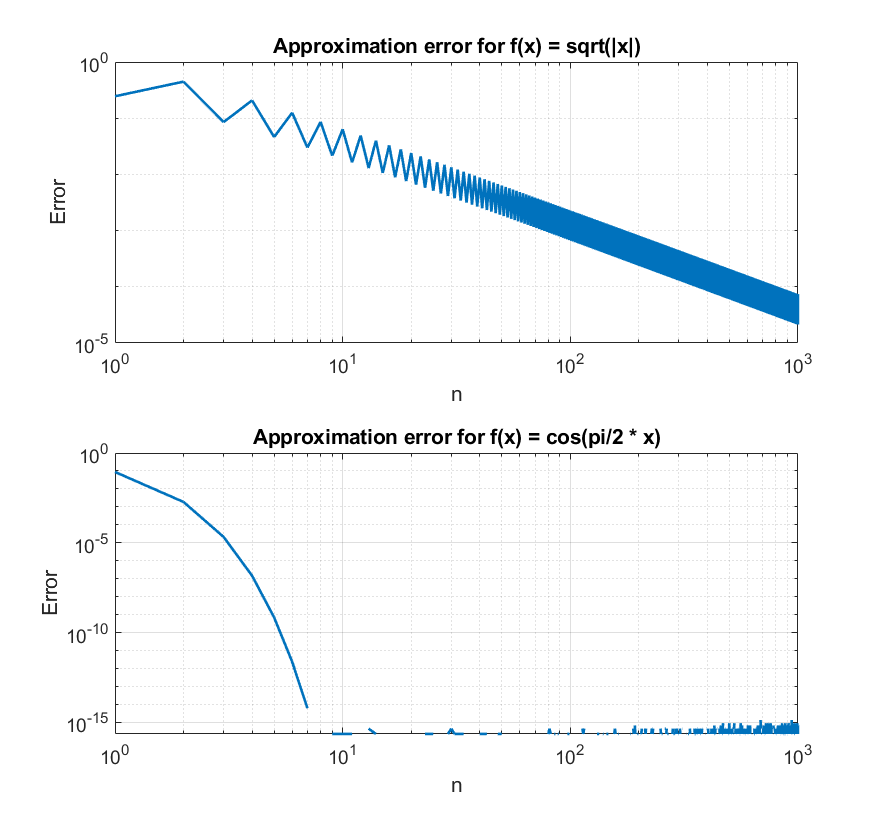
\includegraphics[scale=0.6]{figure.png}
\end{center}

We see the quadrature rule behaves much better with the second function, which
is $C^\infty$.

\newpage

\begin{Verbatim}[frame=single,
   label=\textsc{Matlab} code - main.m]
% Calculate numerically the roots of the polynomials p_n
r_1 = roots([           1,  0])
r_2 = roots([       2,  0, -1])
r_3 = roots([   4,  0, -3,  0])
r_4 = roots([8, 0, -8,  0,  1])

% Compare with explicit formula
r = @(i, n) cos(pi * (2*i + 1)/(2*(n + 1)));
rs = @(n) r((0:n)', n);
xs_1 = rs(0)
xs_2 = rs(1)
xs_3 = rs(2)
xs_4 = rs(3)

% Define quadrature rule
Q = @(f, n) sum(pi/(n + 1)*f(rs(n)));
% MATLAB numerical integration for comparison
w = @(x) 1./sqrt(1 - x.^2);
I = @(f) integral(@(x) f(x).*w(x), -1, 1, 'AbsTol', 1e-16);
% Calculate error in quadrature rule
err = @(f, n) abs(Q(f, n) - I(f));

% Functions we want to integrate
f_1 = @(x) sqrt(abs(x));
f_2 = @(x) cos(pi/2 * x);
ns = 1:1000;
errs_1 = arrayfun(@(n) err(f_1, n), ns);
errs_2 = arrayfun(@(n) err(f_2, n), ns);

% Plot errors on a graph
subplot(2, 1, 1);
loglog(ns, errs_1, 'LineWidth', 2);
xlabel('n');
ylabel('Error')
title('Approximation error for f(x) = sqrt(|x|)');
set(gca, 'FontSize', 14);
grid on;
subplot(2, 1, 2);
loglog(ns, errs_2, 'LineWidth', 2);
xlabel('n');
set(gca, 'FontSize', 14);
ylabel('Error')
title('Approximation error for f(x) = cos(pi/2 * x)');
grid on;
\end{Verbatim}

\end{document}
